\documentclass[journal]{IEEEtran}
\usepackage{graphicx}
\usepackage{booktabs}
\usepackage{multirow}
\usepackage{amsmath,amssymb}
\usepackage{url}
\usepackage{xcolor}
\usepackage{microtype}
\usepackage{array}
\usepackage[hidelinks]{hyperref}
\graphicspath{{figures/}}

% Float-placement tuning so two-column figures share pages with text
\renewcommand{\topfraction}{0.92}
\renewcommand{\bottomfraction}{0.6}
\renewcommand{\textfraction}{0.07}
\renewcommand{\floatpagefraction}{0.7}
\renewcommand{\dbltopfraction}{0.92}
\renewcommand{\dblfloatpagefraction}{0.75}
\setcounter{topnumber}{3}
\setcounter{dbltopnumber}{2}
\setcounter{totalnumber}{5}

% Shorthands for the two shipped chunk families
\newcommand{\cfine}{\textup{c1-1}}
\newcommand{\ccoarse}{\textup{c3-3}}

\begin{document}
\linespread{0.96}\selectfont

\title{Jev-Routed Temporal Granularity with Recovery and Hysteresis for Causal Video Generation}

\author{Hossen~Md~Jisan%
\thanks{H.~M.~Jisan is with the Department of Artificial Intelligence, Nanjing University of Information Science and Technology (NUIST), Nanjing, China (e-mail: jisanahammed1952@gmail.com).}%
\thanks{Code, locked protocols, calibration freezes, and all audit artifacts are openly available at \url{https://github.com/j1s4nn/jev-adaptive-granularity-WM} so that every reported experiment can be independently reproduced.}%
\thanks{Manuscript prepared October 2026. Formatted for \emph{IEEE Transactions on Circuits and Systems for Video Technology} (TCSVT).}}

\markboth{IEEE Transactions on Circuits and Systems for Video Technology (submission draft)}{Jisan: Jev-Routed Temporal Granularity with Recovery and Hysteresis for Causal Video Generation}

\maketitle

\begin{abstract}
Causal video generators produce a rollout one temporal chunk at a time, which invites a simple efficiency idea: spend fine per-frame computation only where a segment is hard, and use cheaper coarse chunks, or even reuse, elsewhere. Realizing this idea requires three preconditions that are usually assumed rather than measured: a mode that is genuinely cheaper on the deployment hardware, a signal that predicts hard segments before generation, and an independent endpoint that certifies the trade. This paper audits all three on Causal-rCM, a Wan2.1-1.3B text-to-video causal diffusion model, pairing a frame-wise mode (\cfine) with a chunk-3 mode (\ccoarse) and a near-zero-cost hold mode, and routing among them with a two-threshold controller with hysteresis and forced recovery. The cost precondition is hardware-conditional: on a Tesla T4 each coarse forward is $3.01\times$ a fine forward against a $2.33\times$ break-even point, so coarse is never cheaper; on an A100-80GB the ratio falls to $1.60$--$1.75$ and coarse is $1.46\times$ faster in diffusion-transformer (DiT) time. A preregistered hand-crafted uncertainty signal fails on 72 locked held-out cases (area under the receiver operating characteristic curve, AUROC, $0.491$), whereas a text-only System One decision model (Jev) reaches AUROC $0.788$ [$0.575,0.946$] at $0.67$\,s per decision, off the GPU. Recovery and hysteresis cut switches from $0.50$ to $0.38$ on the T4 and from $0.92$ to $0.50$ under signal noise on the A100 without worsening regret, and switching carries a measurable seam cost. On 24 fresh A100 prompts, a single-decision Jev policy saves $1.78$\,s of DiT time and $7.39$\,s of total time (both significant) at a small significant $-0.020$ CLIP subject-consistency cost: a genuine, hardware-conditional trade-off, not universal dominance. Negative and failed experiments are preserved as evidence.
\end{abstract}

\begin{IEEEkeywords}
Video generation, world models, diffusion distillation, adaptive computation, temporal granularity, hysteresis control, uncertainty estimation, efficient inference.
\end{IEEEkeywords}

\section{Introduction}
\IEEEPARstart{C}{ausal} video generation with diffusion transformers has become the dominant paradigm for streaming video synthesis and interactive world models, in which frames must be produced one chunk after another under a hard latency budget~\cite{zhengCausalrCMUnifiedTeacherForcing2026,huangSelfForcingBridging2025,zhuCausalForcingAutoregressive2026a,zhaoCausalForcingScalable2026a,aiMAGI1AutoregressiveVideo2025,zhaoMinWMFullStackOpenSource2026a}. Because each chunk is generated conditioned on previously generated context, the rollout invites a natural efficiency idea: not all segments are equally difficult, so one may switch between an expensive \emph{fine} mode (one latent frame per chunk) and a cheaper \emph{coarse} mode (several latent frames per chunk) at run time, deciding from a signal available \emph{before} the segment is generated. This is the video analogue of adaptive computation in recognition networks~\cite{gravesAdaptiveComputationTime2017,teerapittayanonBranchyNetFastInference2017,wangSkipNetLearningDynamic2018} and of dynamic step allocation in autoregressive video diffusion~\cite{leDSADynamicStep2026}, and it complements work that adapts the video \emph{tokenization} itself~\cite{liLearningAdaptiveTemporally2025,xiongEVATokAdaptiveLength2026,yuanDLFRVAEDynamicLatent2025,zhongVFRTokVariableFrame2025}.

The appeal is a better quality--compute frontier than either fixed mode. The premise, however, rests on three preconditions that are easy to conflate and rarely audited together:
\begin{enumerate}
\item[(P1)] \textbf{Cost.} The coarse mode must be cheaper in wall-clock time at usable quality \emph{on the deployment hardware}---fewer denoising steps do not imply lower latency when each step becomes heavier.
\item[(P2)] \textbf{Signal.} Some quantity available before generation must identify the segments where coarse generation would hurt.
\item[(P3)] \textbf{Endpoint.} The quality gain or loss must be certified by an endpoint independent of the modes being compared; an internal reference can silently favor one family.
\end{enumerate}

\subsection{Research Questions}
We organize the audit around four research questions, referred to throughout the paper by number.

\textbf{RQ1 (Signal).} Can a quantity measured \emph{before} a segment is generated predict whether coarse generation would be unsafe for that segment, better than chance and better than hand-crafted statistics of the pre-decision context?

\textbf{RQ2 (Cost--quality trade-off).} Is there a real wall-clock versus quality trade-off from switching temporal granularity online, and is that trade-off conditional on the deployment hardware?

\textbf{RQ3 (Switching control).} Do hysteresis and forced recovery reduce the number of mode switches without worsening rollout regret, and is there a directly measurable quality cost at switch boundaries (a \emph{seam})?

\textbf{RQ4 (Monotonicity).} Is the fine-versus-coarse benefit monotone in the pre-generation signal, so that a threshold on that signal is well posed?

The four questions map onto the three preconditions: RQ1 tests P2, RQ2 tests P1, RQ3 tests the mechanism that stabilizes a controller once P1 and P2 hold, and RQ4 tests whether a scalar threshold is even the right decision rule.

\subsection{System Overview and Contributions}
We audit the preconditions end to end on a real system: Causal-rCM~\cite{zhengCausalrCMUnifiedTeacherForcing2026}, a Wan2.1-T2V-1.3B-480p causal diffusion model~\cite{wan2025wan}, using its two shipped chunk families, frame-wise \cfine{} and chunk-3 \ccoarse, plus a near-zero-cost \emph{hold} mode that copies the previous latent frame. Routing is performed per segment by a two-threshold controller with a hysteresis band and a forced recovery window, driven either by hand-crafted signals (residual, optical-flow warp, motion, complexity) or by the \emph{Jev} System One decision model, a text-only oracle that answers typed difficulty, drift-risk, and motion-class questions from a caption of the pre-decision context frame. The audit runs on two GPUs with very different compute characters, a 16\,GB Tesla T4 and an A100-SXM4-80GB, because the cost precondition turned out to be a property of the hardware, not of the model.

Our findings are deliberately evidence-preserving. On the T4 the coarse family has about $3\times$ fewer neural function evaluations (NFEs) but each forward is about $3\times$ heavier, so it is not cheaper; the preregistered signal test fails outright (held-out AUROC $0.491$); and an online warp-threshold policy degenerates to a per-prompt fixed choice at $2.2\times$ the cost of the best fixed policy. On the A100 the cost ordering reverses (coarse is $1.46\times$ faster in DiT time) but the independent endpoint still rejects the hand-crafted policy, because it trades subject consistency for DiT seconds and its own signal decoding erases the total-time gain.

Our contributions are:
\begin{enumerate}
\item A paired T4/A100 audit showing that the fine/coarse \emph{cost inversion is hardware-conditional} (per-forward ratio $3.01$ vs.\ $1.60$ against a $2.33$ break-even point), resolving an apparent contradiction between NFE counts and wall-clock time (Section~\ref{sec:cost}, RQ2).
\item A preregistered \emph{negative} result for hand-crafted pre-generation signals (288 held-out segments), and a positive replacement: the Jev System One oracle at AUROC $0.788$ [$0.575,0.946$], computed off the generation path (Section~\ref{sec:signal}, RQ1).
\item A recovery-plus-hysteresis controller ablation on both GPUs with a directly measured \emph{seam cost} at switch boundaries (Section~\ref{sec:rq3}, RQ3).
\item A confirmatory 24-prompt A100 study with prompt-paired bootstrap confidence intervals establishing a \emph{trade-off, not dominance}, for Jev-routed generation (Section~\ref{sec:phase3}, RQ2).
\item An exploratory monotonicity analysis showing that the fine-versus-coarse benefit is monotone in the Jev difficulty signal on the T4 but flat on the A100 diagnostic split, tying RQ4 to RQ1 and to the choice of endpoint (Section~\ref{sec:rq4}, RQ4).
\end{enumerate}

We make no claim of universal adaptive superiority. The value of the study is a reproducible account of when the three preconditions hold, what breaks when they do not, and a working routing mechanism---Jev plus recovery and hysteresis---for the regime in which they do.

\section{Related Work}
\label{sec:related}

\subsection{Causal and few-step autoregressive video diffusion}
Autoregressive video diffusion replaces bidirectional attention over a full clip with causal attention over generated history, enabling streaming and interactive synthesis. Self Forcing closes the train--test gap by training on the model's own rollouts~\cite{huangSelfForcingBridging2025}; Causal Forcing and Causal Forcing++ systematize few-step autoregressive distillation for real-time interactive generation, the latter explicitly contrasting frame-wise and chunk-wise regimes~\cite{zhuCausalForcingAutoregressive2026a,zhaoCausalForcingScalable2026a}; minWM provides a full-stack open framework~\cite{zhaoMinWMFullStackOpenSource2026a}; MAGI-1 scales chunk-wise generation~\cite{aiMAGI1AutoregressiveVideo2025}. Causal-rCM unifies teacher-forcing consistency distillation with self-forcing refinement and ships frame-wise and chunk-wise students of Wan2.1~\cite{zhengCausalrCMUnifiedTeacherForcing2026,wan2025wan}; we build directly on its released \cfine{} and \ccoarse{} checkpoints. Related designs include Diagonal Distillation~\cite{liuStreamingAutoregressiveVideo2026}, Flex-Forcing, which also explores device-budget-aware inference~\cite{maFlexForcingUnifiedAutoregressive2026}, Next Forcing~\cite{xuNextForcingCausal2026}, and semi-autoregressive or non-quantized variants~\cite{renNextBlockPrediction2025,dengAutoregressiveVideoGeneration2025}. All fix a single temporal granularity at deployment; we treat granularity as a per-segment decision.

\subsection{Adaptive computation and adaptive tokenization}
Allocating inference effort by input difficulty is classical: adaptive computation time~\cite{gravesAdaptiveComputationTime2017}, early exits~\cite{teerapittayanonBranchyNetFastInference2017}, and learned layer skipping~\cite{wangSkipNetLearningDynamic2018}. In video generation, DSA allocates denoising steps dynamically along an autoregressive rollout~\cite{leDSADynamicStep2026}, the closest published point to our fine/coarse regimes, but it does not switch the chunking mode nor study the hardware dependence of the step--latency map. A parallel line adapts the tokenizer---temporally causal one-dimensional tokenization~\cite{liLearningAdaptiveTemporally2025}, adaptive-length tokens~\cite{xiongEVATokAdaptiveLength2026}, dynamic latent frame rate~\cite{yuanDLFRVAEDynamicLatent2025}, and variable-frame-rate tokenizers~\cite{zhongVFRTokVariableFrame2025}---changing granularity at the representation level and offline; we keep the released tokenizer fixed and route among shipped inference modes online.

\subsection{Error accumulation, surprise, and switching control}
Long rollouts accumulate error, and several works respond with content-adaptive mechanisms: entropy-guided guard sampling~\cite{hanEntropyGuidedKGuard2026}, surprise-based hierarchical chunking~\cite{iiyamaSUNTAHierarchical2026}, surprise-driven memory~\cite{shiSurpriseForcingWhat2026}, state-adaptive scheduling~\cite{sunSANTSStateAdaptiveScheduler2026}, and context-aware mixture-of-experts for long horizons~\cite{shangLongScapeAdvancingLongHorizon2025}. LongScape additionally uses action-guided variable-length chunking in an embodied setting; we instead drive granularity from a pre-generation signal with an explicit recovery window. DASH-OPD introduces discrepancy-aware switching \emph{with hysteresis} for on-policy distillation~\cite{xiaDASHOPDDiscrepancy2026}; our controller reuses the same classical two-threshold band but applies it at inference time to granularity selection, adds forced recovery, and directly measures the seam cost that hysteresis is meant to amortize.

\subsection{Caching, memory, and serving efficiency}
Complementary savings come from reusing computation rather than choosing modes: content-aware key--value selection~\cite{caiFocusedForcingContentAware2026}, flow caching~\cite{maFlowCachingAutoregressive2026}, motion-aware caching~\cite{xuMotionAwareCachingEfficient2026}, key--value cache quantization~\cite{ranganathKVCacheQuantization2026}, and serving-level resource management~\cite{xiaAdaptiveResourceManagement2026}. These are orthogonal to granularity routing and composable with it.

\subsection{Evaluation endpoints}
Our independent endpoints use CLIP ViT-B/32 subject consistency and text alignment~\cite{radford2021clip}, following the subject-consistency dimension popularized by VBench~\cite{huang2024vbench}, plus a classical optical-flow suite; context frames are captioned with BLIP~\cite{li2022blip} for the oracle input. The hardware contrast is mediated by attention kernels---SDPA on the Turing T4 versus FlashAttention on Ampere-class GPUs~\cite{dao2022flashattention}---which is why the cost precondition is hardware-conditional.

\textbf{Positioning.} Prior systems make generation cheap, smooth, or interactive, and efficiency work adapts compute, tokens, cache, or serving. To our knowledge none decides \emph{per segment, online, which temporal granularity to run next} from a signal computed \emph{before} generation, none adds a recovery mechanism when that signal fails, and none audits whether the underlying cost premise holds across hardware. That audit plus the working mechanism is the contribution here.

\section{Background: Modes and the Operating-Point Trap}
\label{sec:background}

Causal-rCM generates a rollout over latent-frame chunks $[\text{first\_chunk} \mid \text{chunk}_1 \mid \text{chunk}_2 \mid \dots]$, each chunk attending causally to its predecessors~\cite{zhengCausalrCMUnifiedTeacherForcing2026}. The two shipped families are \cfine{} (one initial latent frame, then one-frame chunks) and \ccoarse{} (three initial latent frames, then three-frame chunks), each with documented one-, two-, and four-step midpoint schedules. A $k$-frame chunk mode performs one transformer forward per denoising step \emph{per chunk}, so its NFE count is divided by $k$ relative to the frame-wise family, while each forward processes $k$ times as many latent frames.

This definition creates an \emph{operating-point trap}. An early comparison paired \cfine{} in its one-step regime against \ccoarse{} in its four-step regime and found coarse slower in all 72/72 held-out cases (DiT $53.4$\,s vs.\ $21.6$\,s), which naively reads as ``coarse is broken'' but is in fact a schedule mismatch. The trap generalizes: coarse is cheaper in wall-clock DiT time only if
\begin{equation}
\frac{s_{\text{fwd}}^{\ccoarse}}{s_{\text{fwd}}^{\cfine}} \;<\; \frac{\mathrm{NFE}_{\cfine}}{\mathrm{NFE}_{\ccoarse}},
\label{eq:breakeven}
\end{equation}
where the right-hand side is set by the chosen schedules. For the one-step regimes used throughout (NFE $19$ vs.\ $8.33$ at 57 frames, and $21$ vs.\ $9$ under noisy context), the break-even ratio is $2.33$. The measured per-forward ratio is $3.01$ on the T4 but $1.60$ on the A100 (Section~\ref{sec:cost}): the same model pair lies on opposite sides of \eqref{eq:breakeven} on different GPUs, because the Ampere-class A100 with FlashAttention~\cite{dao2022flashattention} amortizes the heavier three-frame forward far better than the Turing T4 with SDPA. Causal-rCM itself reports non-monotone quality versus refinement for frame-wise one- and two-step schedules~\cite{zhengCausalrCMUnifiedTeacherForcing2026}, which additionally motivates testing whether the fine-versus-coarse benefit is monotone in uncertainty (Section~\ref{sec:rq4}).

\section{Method: Jev-Routed Granularity Control}
\label{sec:method}

\begin{figure*}[!t]
\centering
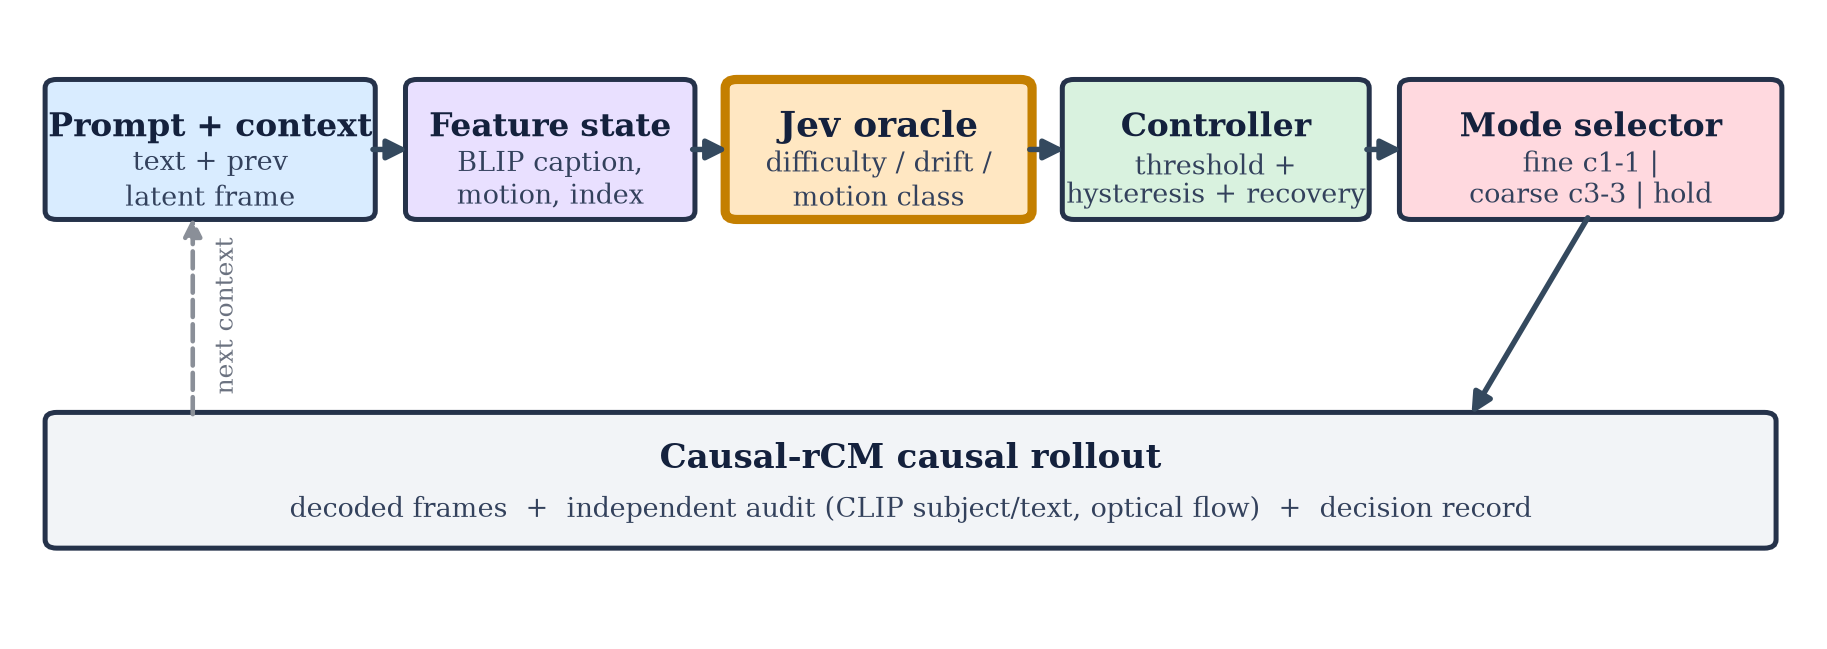
\includegraphics[width=0.62\textwidth]{architecture.png}
\caption{Pre-generation routing and causal rollout. For each segment, a feature state (prompt, BLIP caption of the pre-decision context frame, segment index, motion statistics) is sent to the Jev oracle, which returns typed difficulty, drift-risk, and motion-class outputs. The controller state (threshold, hysteresis band, recovery counter) maps these to an action in $\{$fine \cfine, coarse \ccoarse, hold$\}$, and the selected mode executes the next causal segment. Every decision is recorded with its generated frames, independent quality measures, timing, and switch-boundary cost; all measurements are prompt-paired, and the internal \cfine{} reference is diagnostic only.}
\label{fig:arch}
\end{figure*}

\subsection{Decision structure}
\label{sec:decision}
Figure~\ref{fig:arch} summarizes the system. Rollouts use a fixed grid: a shared coarse prefix of three latent frames, followed by $T$ segments of three latent frames each (four segments at a 57-frame horizon). Before each segment $t$, the controller selects an action
\begin{equation}
a_t \in \{\text{fine } (\cfine),\ \text{coarse } (\ccoarse),\ \text{hold}\},
\end{equation}
where hold copies the previous latent frame at near-zero DiT cost. The action conditions on a pre-generation state only; nothing from the not-yet-generated segment is used.

\subsection{The Jev System One oracle}
\label{sec:jev}
Hand-crafted signals from the pre-decision context (residual, warp, motion, complexity; Section~\ref{sec:signal}) failed the preregistered held-out test, so we replace them with an external \emph{System One} decision model, Jev (TypeSafe API, model identifier \texttt{jev-latest}), queried once per decision with a composite typed prompt. The state sent per segment is
\begin{equation}
s_t = (\text{prompt},\ \text{caption}(x_{t-1}),\ t,\ \bar{m}_t,\ \bar{w}_t),
\end{equation}
where $\text{caption}(x_{t-1})$ is a BLIP caption~\cite{li2022blip} of the last decoded pre-decision frame and $\bar{m}_t,\bar{w}_t$ are recent motion-magnitude and warp statistics. The oracle returns three typed outputs: a numeric drift risk $r_t \in [0,1]$ (continuous risk score: whether a coarse chunk would drift or become temporally inconsistent), a difficulty score $d_t$ on a five-level ordinal scale mapped to a number (score type), and a motion class $q_t \in \{$static, moderate, fast, scene\_change$\}$ (choice type). Mean latency is $0.672$\,s per decision ($n{=}80$), off the GPU and off the DiT path; the hand-crafted warp signal, in contrast, requires a VAE decode of the context ($\approx$156\,s at 57 frames on the T4). Retries use exponential backoff with a 40\,s timeout; the API key is read from the environment and never committed. We disclose the methodological risk: Jev is external, proprietary, and versioned (Section~\ref{sec:limitations}).

\subsection{Controller: threshold, hysteresis, recovery}
\label{sec:controller}
Given a scalar signal $u_t$ (the warp statistic or the Jev difficulty score), a threshold controller switches mode when $u_t$ crosses a decision threshold $\tau$. Two mechanisms stabilize it. \emph{Hysteresis} maintains a band $\Lambda = \tau_{\text{high}} - \tau_{\text{low}}$ around the operating point: the mode changes only when the signal exits the band, not on every crossing of $\tau$. \emph{Recovery} forces the fine mode for $R$ consecutive segments after a detected quality spike, then re-arms. Formally, with potential $\Psi_t = u_t + \lambda \Delta a_t$ (we set $\lambda{=}0$ throughout, since no action-conditioned checkpoint is available),
\begin{equation}
a_t =
\begin{cases}
\text{fine}, & \Psi_t \ge \tau_{\text{high}} \ \text{or recovery active},\\
\text{coarse/hold}, & \Psi_t \le \tau_{\text{low}},\\
a_{t-1}, & \text{otherwise}.
\end{cases}
\label{eq:policy}
\end{equation}
Thresholds are calibrated on a development split only: for the warp controller, $\tau$ is the pooled development median ($4.416$), the band is $\Lambda = 2\sigma_u$ with $\sigma_u = 3.915$, and $R{=}2$; for the Jev router, the motion-class rule calibrated on development answers is
\begin{equation}
\begin{aligned}
\text{static} &\rightarrow \text{hold},\qquad
\text{moderate} \rightarrow \text{coarse},\\
\text{fast}/\text{scene}&\text{\_change} \rightarrow \text{fine},
\end{aligned}
\label{eq:routing}
\end{equation}
with a difficulty-threshold gate ($\tau_{\text{Jev}} = 1.72$, development Youden index $0.524$) for the difficulty-driven variant. Over the 32 development decisions, rule \eqref{eq:routing} assigns 16 coarse, 9 hold, and 7 fine actions---the modes are genuinely mixed, not degenerate.

Two structural properties motivate the design. \emph{Oscillation bound:} for additive signal noise $|\epsilon| \le \sigma$, a two-threshold controller's per-step switching probability is bounded by $\Pr[|u + \epsilon - \tau| \ge \Lambda/2]$, so $\Lambda \ge 2\sigma$ eliminates noise-only crossings---the regime the noisy-arm ablation stresses (Section~\ref{sec:rq3}). \emph{Fixed-mode suboptimality:} if coarse attains lower distance than fine on safe segments and vice versa on unsafe ones, with both sets non-empty, the per-segment oracle beats either fixed policy, and any router whose selection error is below a derived bound beats fixed fine. We record honestly that the second proposition's parameter regime was not reachable in the deployed setting; it is motivation, not a guarantee.

\section{Experimental Setup}
\label{sec:setup}

\textbf{Model and software.} Causal-rCM Wan2.1-T2V-1.3B-480p~\cite{zhengCausalrCMUnifiedTeacherForcing2026,wan2025wan}, checkpoints \texttt{c1-1\_step2}, \texttt{c1-1\_step4}, \texttt{c3-3\_step2}, \texttt{c3-3\_step2\_noisy\_ctx}, \texttt{c3-3\_step4}; umT5-XXL text encoding and the Wan2.1 VAE; guidance $5.0$, shift $8.0$, 480$\times$832 at 16\,fps. Inference is fp16 with the verified single-file recipe (patched dtype, local tokenizer, DiT freed before VAE decode, \texttt{expandable\_segments}); PyTorch SDPA attention on the T4, FlashAttention-2 on the A100~\cite{dao2022flashattention}. All A100 runs pin upstream commit \texttt{ed3cb14dd936f92cdc9f9381af7369991509b41f}.

\textbf{Hardware.} A Kaggle Tesla T4 (16\,GB) and a Google Colab A100-SXM4-80GB. The two machines bracket the deployment regimes of interest: a memory- and throughput-limited Turing card versus an Ampere datacenter card.

\textbf{Endpoints.} (i) \emph{Internal diagnostic:} decoded-pixel $L_1$ distance (refL1) to a \cfine{} four-step reference at matched prompt, seed, and noise. Because the reference is itself from the fine family, this endpoint can flatter either mode and is never used alone. (ii) \emph{Independent:} CLIP ViT-B/32 subject consistency and text alignment~\cite{radford2021clip,huang2024vbench}. (iii) \emph{Classical temporal suite:} optical-flow backward-warp residual, frame-difference $L_1$, flow magnitude, and histogram correlation.

\textbf{Prompts and splits.} Three development prompts drive the mode sweeps; the preregistered signal test locks 12 calibration and 24 held-out prompts with seeds $17/29/41$ (72 held-out cases, 288 scored segments); eight fresh VBench-derived prompts~\cite{huang2024vbench} spanning object, scene, motion, and human-action strata drive the T4 online, controller, monotonicity, and Jev studies; the A100 arm uses fresh manifests of 12 prompts (online policies, controller ablation) and 24 fresh prompts (confirmatory study). Development, calibration, and evaluation splits are disjoint.

\textbf{Protocols and statistics.} The master protocol locks the reference construction, the 45/57/81-frame segment grids, the distance fallback, the calibration split, matched-budget baselines (fixed, random-50, alternating-50), grouped prompt$\times$seed bootstrap intervals, and the preservation of negative results. The locked adaptive-selection criterion requires an adaptive policy to beat fixed fine \emph{and} random same-budget on the independent endpoint at lower measured DiT cost with grouped intervals excluding zero. The A100 protocol adds the hold and latent-refresh policies and a 10{,}000-resample prompt-paired bootstrap against fixed fine.

\section{Results}
\label{sec:results}

\subsection{Mode cost is hardware-conditional (RQ2)}
\label{sec:cost}

\begin{figure*}[!t]
\centering
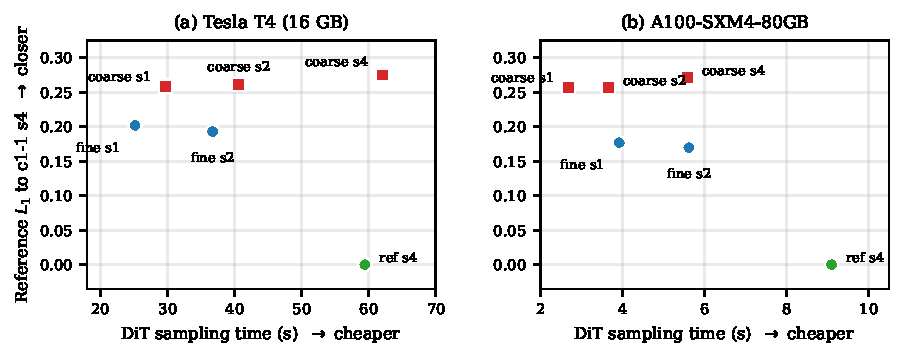
\includegraphics[width=0.90\textwidth]{fig_cost_pareto.pdf}
\caption{Six-mode cost--quality sweep on (a) the Tesla T4 and (b) the A100-80GB. Fewer NFEs do not imply lower DiT time: on the T4 every coarse mode sits above and to the right of fine \cfine{} s1, while on the A100 the coarse family occupies a cheaper, less accurate frontier point. The internal refL1 axis is diagnostic (the reference is a fine-family rollout).}
\label{fig:cost}
\end{figure*}

\begin{table}[!t]
\centering
\caption{Six-mode sweep on the Tesla T4 (45/57/81-frame grid, 3 development prompts, 39 scored pairs). DiT is the mode-dependent cost; VAE decode is mode-independent. refL1 is the internal diagnostic distance to \cfine{} s4.}
\label{tab:t4sweep}
\renewcommand{\arraystretch}{1.12}
\footnotesize
\setlength{\tabcolsep}{3pt}
\begin{tabular}{@{}lrrrrr@{}}
\toprule
Mode & DiT (s) & VAE (s) & Total (s) & NFE & refL1 \\
\midrule
ref \cfine{} s4   & 59.42 & 155.7 & 227.8 & 64.0 & 0.0000 \\
fine \cfine{} s1  & \textbf{25.16} & 156.5 & \textbf{194.5} & 19.0 & \textbf{0.2019} \\
fine \cfine{} s2  & 36.73 & 155.7 & 205.5 & 34.0 & 0.1930 \\
coarse \ccoarse{} s4 & 62.05 & 155.7 & 232.1 & 21.3 & 0.2750 \\
coarse \ccoarse{} s2 & 40.63 & 155.6 & 210.5 & 12.7 & 0.2615 \\
coarse \ccoarse{} s1 & 29.72 & 155.9 & 197.6 & \textbf{8.3} & 0.2588 \\
\bottomrule
\end{tabular}
\end{table}

\begin{table}[!t]
\centering
\caption{Six-mode sweep on the A100-80GB with real umT5 encoding and VAE decode (9 cases). The cost ordering of Table~\ref{tab:t4sweep} reverses; coarse remains less accurate on every quality measure.}
\label{tab:a100sweep}
\renewcommand{\arraystretch}{1.12}
\footnotesize
\setlength{\tabcolsep}{3pt}
\begin{tabular}{@{}lrrrrr@{}}
\toprule
Mode & DiT (s) & VAE (s) & Total (s) & NFE & refL1 \\
\midrule
ref \cfine{} s4   & 9.10 & 2.52 & 18.40 & 64.0 & 0.0000 \\
fine \cfine{} s1  & 3.92 & 2.38 & 12.95 & 19.0 & \textbf{0.1769} \\
fine \cfine{} s2  & 5.62 & 2.38 & 14.68 & 34.0 & 0.1697 \\
coarse \ccoarse{} s4 & 5.58 & 2.39 & 14.71 & 21.3 & 0.2712 \\
coarse \ccoarse{} s2 & 3.65 & 2.39 & 12.59 & 12.7 & 0.2571 \\
coarse \ccoarse{} s1 & \textbf{2.69} & 2.38 & \textbf{11.66} & \textbf{8.3} & 0.2575 \\
\bottomrule
\end{tabular}
\end{table}

\begin{table}[!t]
\centering
\caption{Cost precondition across hardware and context regime. The per-forward ratio is compared with the schedule break-even ratio of \eqref{eq:breakeven} (2.33 for the one-step regimes). Coarse is cheaper only on the A100, where the ratio falls below break-even.}
\label{tab:costpre}
\renewcommand{\arraystretch}{1.12}
\footnotesize
\setlength{\tabcolsep}{4pt}
\begin{tabular}{@{}lrrrr@{}}
\toprule
Setting & fine s/fwd & coarse s/fwd & ratio & cheaper? \\
\midrule
T4, clean context      & 1.32  & 3.58  & 3.01 & no \\
T4, noisy context      & 0.71  & 2.10  & 2.94 & no \\
A100, timing arm       & 0.125 & 0.200 & 1.60 & yes \\
A100, full-decode arm  & 0.112 & 0.196 & 1.75 & yes \\
\bottomrule
\end{tabular}
\end{table}

Table~\ref{tab:t4sweep} and Fig.~\ref{fig:cost}(a) give the T4 sweep. The \ccoarse{} family has about $3\times$ fewer NFEs, but each forward is about $3\times$ heavier ($3.58$ vs.\ $1.32$\,s per NFE at the one-step regimes), so coarse is \emph{not} cheaper in wall-clock DiT time, and it is consistently farther from the reference. Fine \cfine{} s1 dominates every coarse mode on both axes. Independent endpoints agree: coarse modes are less temporally smooth (warp $0.0334$--$0.0336$ vs.\ $0.0280$ for fine s1) with no consistent CLIP advantage. A noisy-context variant (reusing the final denoising forward as the next chunk's context) roughly halves DiT time for \emph{both} families and therefore creates no coarse advantage; we report it as a replicated upstream efficiency trick, not as our novelty.

The same sweep on the A100 reverses the cost clause (Table~\ref{tab:a100sweep}, Fig.~\ref{fig:cost}(b)). The coarse/fine per-forward ratio drops from $3.01$ (T4) to $1.60$ (timing-only) and $1.75$ (real-decode arm), below the $2.33$ break-even point of \eqref{eq:breakeven}: coarse \ccoarse{} s1 is $1.46\times$ faster in DiT time than fine s1 ($2.69$ vs.\ $3.92$\,s). Quality moves the other way: refL1 $0.2575$ vs.\ $0.1769$, CLIP subject consistency $0.9880$ vs.\ $0.9890$, temporal warp $0.0329$ vs.\ $0.0226$. VAE decode falls from $\approx$156\,s (T4) to $\approx$2.4\,s and stops dominating the total. \emph{The quality--cost trade-off exists on the A100 and is absent on the T4}: precondition P1 is a property of the GPU. Fig.~\ref{fig:hwscaling} summarizes the rollout latencies and the per-forward ratios against the break-even point; Table~\ref{tab:costpre} collects the per-forward ratios.

\begin{figure*}[!t]
\centering
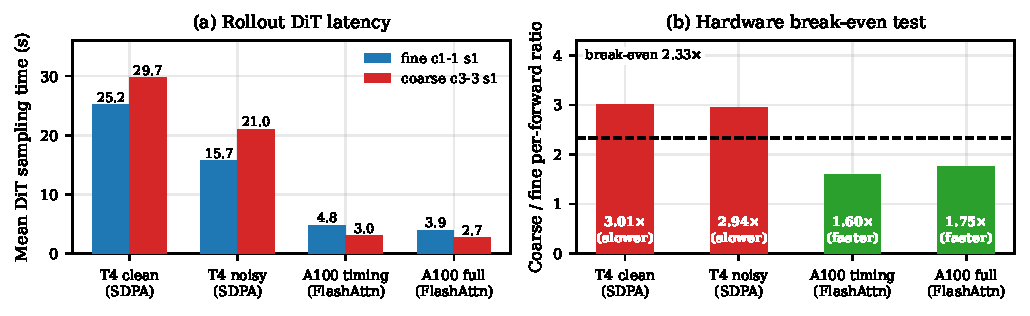
\includegraphics[width=0.90\textwidth]{fig_hw_scaling.pdf}
\caption{Cost precondition across hardware and context regime. (a) Rollout DiT latency for the one-step fine and coarse modes on the T4 (clean and noisy context) and the A100 (timing-only and full-decode arms). (b) The coarse/fine per-forward time ratio against the $2.33$ break-even point; the same model pair lies above break-even on the T4 (coarse slower) and below it on the A100 (coarse faster).}
\label{fig:hwscaling}
\end{figure*}

\subsection{The hand-crafted signal fails; Jev is predictive (RQ1)}
\label{sec:signal}

\begin{figure*}[!t]
\centering
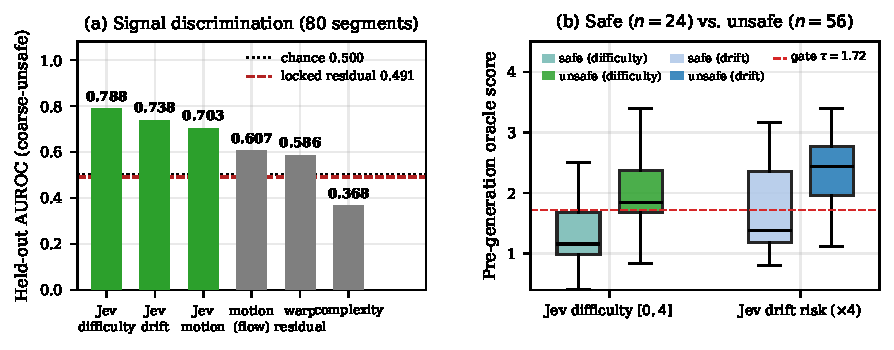
\includegraphics[width=0.84\textwidth]{fig_auroc.pdf}
\caption{Signal discrimination. (a) Held-out AUROC on 80 paired T4 segments (coarse-unsafe label; prompt-grouped 95\% bootstrap CIs are listed in Table~\ref{tab:signal}): the three Jev outputs outperform every hand-crafted signal, the dashed line marks the preregistered residual result ($0.491$), and the dotted line is chance. (b) Score separation of the Jev difficulty and drift outputs between coarse-safe ($n{=}24$) and coarse-unsafe ($n{=}56$) segments, with the calibrated gate.}
\label{fig:auroc}
\end{figure*}

\begin{table}[!t]
\centering
\caption{Held-out AUROC for predicting coarse-unsafe segments. The locked signal study scores 72 held-out cases (288 segments). The Jev audit uses 80 paired segments from 8 fresh prompts; prompt-grouped 95\% CIs, 2{,}000 resamples.}
\label{tab:signal}
\renewcommand{\arraystretch}{1.12}
\footnotesize
\setlength{\tabcolsep}{3pt}
\begin{tabular}{@{}llcc@{}}
\toprule
Study & Signal & AUROC & 95\% CI \\
\midrule
\multirow{4}{*}{Locked}
 & residual   & 0.491 & [0.393, 0.589] \\
 & warp       & 0.454 & [0.343, 0.566] \\
 & motion     & 0.488 & [0.377, 0.600] \\
 & complexity & 0.301 & [0.197, 0.412] \\
\midrule
\multirow{6}{*}{Jev audit (80 seg.)}
 & \textbf{Jev difficulty} & \textbf{0.788} & [0.575, 0.946] \\
  & Jev drift risk          & 0.738 & [0.479, 0.945] \\
 & Jev motion (choice)     & 0.703 & [0.472, 0.873] \\
 & motion (hand-crafted)   & 0.607 & [0.260, 0.857] \\
 & warp (hand-crafted)     & 0.586 & [0.222, 0.836] \\
 & complexity (hand-crafted) & 0.368 & [0.184, 0.562] \\
\bottomrule
\end{tabular}
\end{table}

Table~\ref{tab:signal} and Fig.~\ref{fig:auroc} report the signal audit. The preregistered hypothesis fails on locked data: the residual signal's held-out AUROC is $0.491$, and its paired advantage over the strongest calibration baseline (warp) is $0.0367$ with 95\% CI $[-0.0493, 0.1194]$ including zero. We preserve this as the study's central negative result. Re-labeling the same 80 paired segments (label: coarse regret exceeds fine regret; 56/80 positives) with the Jev oracle reverses the conclusion: Jev difficulty reaches AUROC $0.788$ [$0.575, 0.946$], $+0.180$ over the best hand-crafted signal and $+0.297$ over the preregistered residual, with the interval excluding $0.491$. The signal content, not the label, was the bottleneck. The oracle answers \emph{before} generation in $0.672$\,s, versus a $\approx$156\,s VAE decode for the warp signal on the T4---about $230\times$ cheaper and entirely off the GPU. Precondition P2 is therefore satisfiable, but not by the hand-crafted suite.

\begin{figure}[!t]
\centering
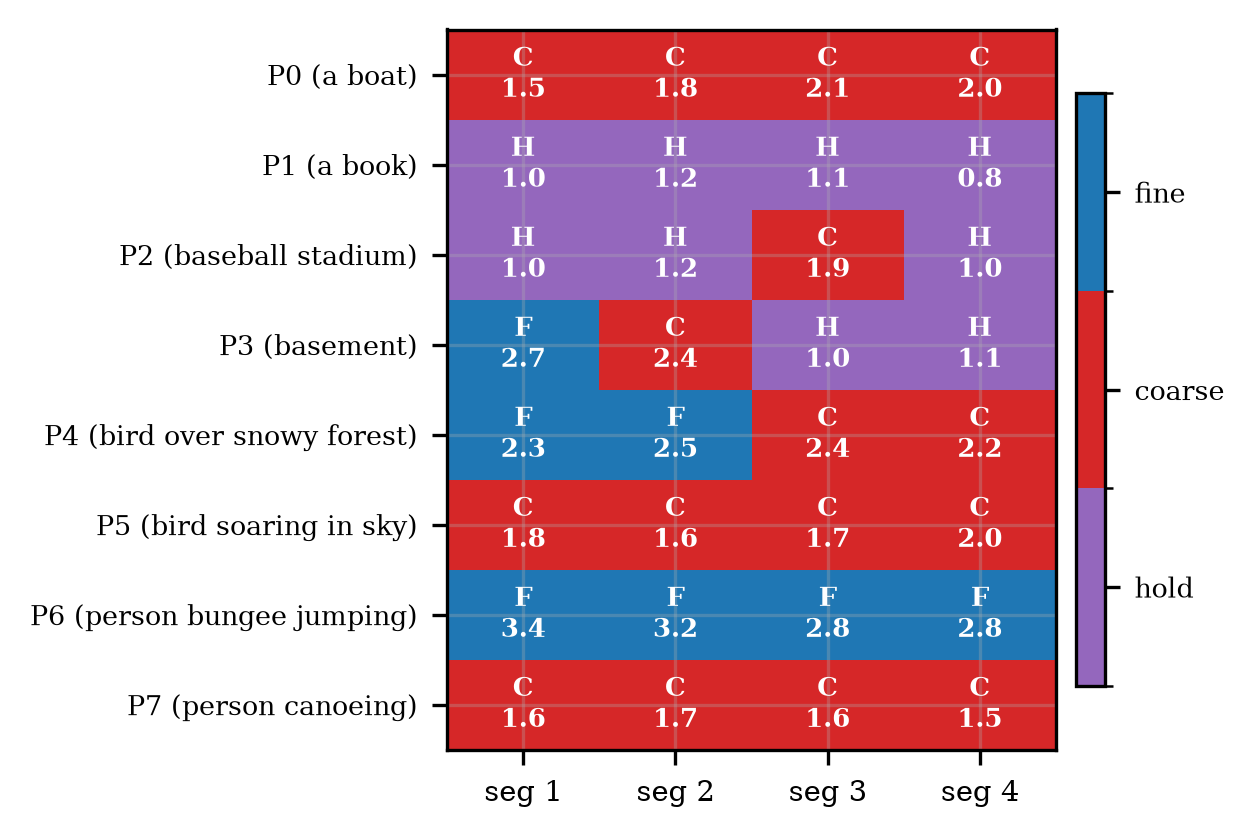
\includegraphics[width=\linewidth]{fig_jev_routing.png}
\caption{Jev routing traces over the eight T4 prompts (57 frames, four segment decisions each). Each cell shows the selected action (F = fine, C = coarse, H = hold) and the oracle's difficulty score. The traces are non-degenerate: static content is held (P1, P2), fast motion is routed to fine (P3, P4, P6), and moderate motion to coarse (P0, P5, P7).}
\label{fig:jevroute}
\end{figure}

Figure~\ref{fig:jevroute} shows the per-segment decisions produced by the motion-class rule \eqref{eq:routing} on the eight T4 prompts: the traces are non-degenerate and interpretable---static prompts are held, fast-motion prompts (a bungee jumper, a bird over snow) are routed to fine, and moderate-motion prompts to coarse.

\subsection{Online routing on the T4: fixed fine dominates}
\label{sec:f4lite}

\begin{figure*}[!t]
\centering
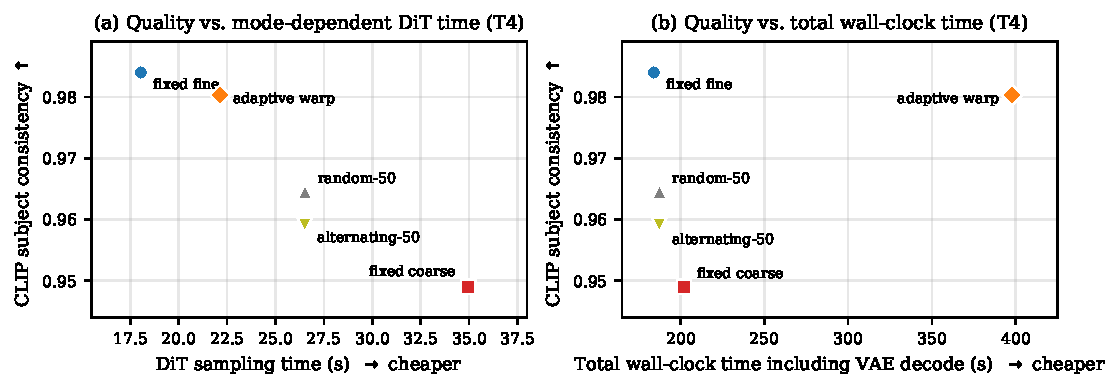
\includegraphics[width=0.90\textwidth]{f4lite_policy_pareto.pdf}
\caption{Budgeted online policies on the T4 (8 fresh prompts, 57 frames): independent CLIP subject consistency against (a) mode-dependent DiT time and (b) total wall-clock including repeated VAE decodes. Fixed fine dominates on both axes; the adaptive warp policy pays $2.9\times$ VAE cost for its signal and never switches within a video.}
\label{fig:f4lite}
\end{figure*}

\begin{figure}[!t]
\centering
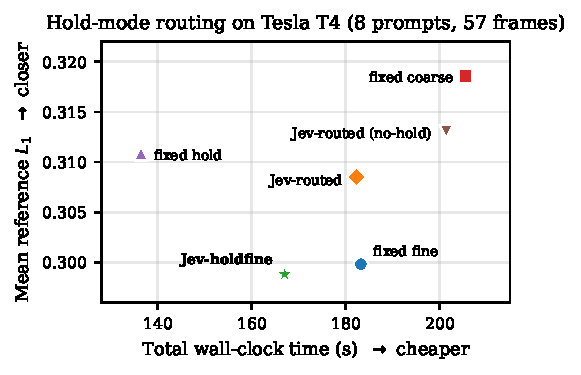
\includegraphics[width=\linewidth]{jev_hold_mode.pdf}
\caption{Hold-mode study on the T4 (8 prompts, 57 frames; internal refL1 vs. total wall-clock). Routing static segments to the near-zero-cost hold mode (Jev-holdfine, star) beats fixed fine on both axes; routing moderate segments to the heavier coarse mode (Jev-routed) does not.}
\label{fig:hold}
\end{figure}

\begin{figure*}[!t]
\centering
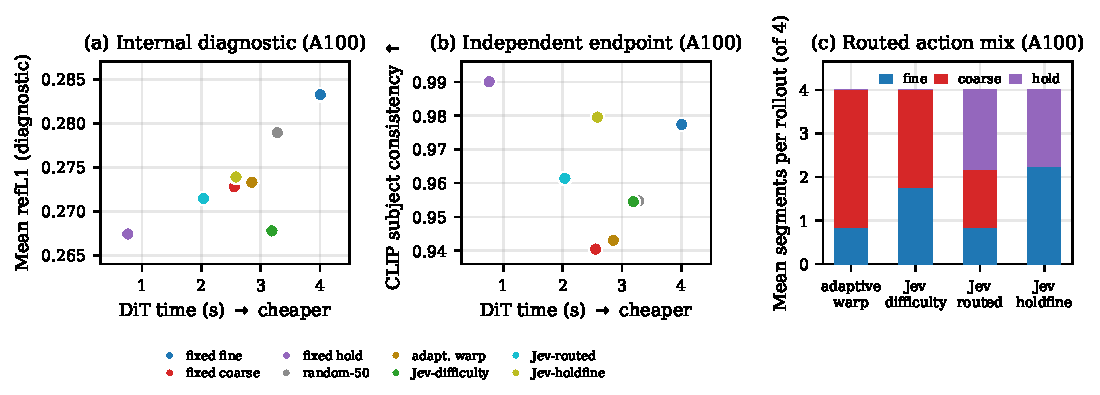
\includegraphics[width=0.90\textwidth]{fig_a100_online.pdf}
\caption{A100 online policies (12 fresh prompts, 57 frames) on (a) the internal refL1 diagnostic, (b) the independent CLIP subject-consistency endpoint, and (c) the mean routed action mix per rollout. The internal reference and the independent endpoint rank the same policies differently: the internal reference flatters coarse-family policies, while the independent endpoint keeps fixed fine and Jev-holdfine on top.}
\label{fig:a100online}
\end{figure*}

\begin{table}[!t]
\centering
\caption{Budgeted online policies on the T4 (8 fresh prompts, 57 frames, one shared coarse prefix then four segment decisions). refL1 is the internal diagnostic; CLIP subject consistency and warp are independent endpoints.}
\label{tab:f4lite}
\renewcommand{\arraystretch}{1.12}
\footnotesize
\setlength{\tabcolsep}{3pt}
\begin{tabular}{@{}lrrrrr@{}}
\toprule
Policy & refL1$\downarrow$ & DiT (s) & Total (s) & CLIP subj.$\uparrow$ & warp$\downarrow$ \\
\midrule
fixed coarse     & 0.3186 & 35.0 & 202.1 & 0.9490 & 0.0733 \\
\textbf{fixed fine} & \textbf{0.2998} & \textbf{18.1} & \textbf{184.1} & \textbf{0.9840} & \textbf{0.0303} \\
random-50        & 0.3102 & 26.5 & 187.5 & 0.9646 & 0.0526 \\
alternating-50   & 0.3058 & 26.5 & 187.3 & 0.9591 & 0.0552 \\
adaptive warp    & 0.2949 & 22.1 & 397.8 & 0.9803 & 0.0429 \\
\bottomrule
\end{tabular}
\end{table}

\begin{table}[!t]
\centering
\caption{Hold-mode routing on the T4 (8 prompts, 57 frames, shared coarse prefix; mode counts are mean actions per rollout out of four).}
\label{tab:hold}
\renewcommand{\arraystretch}{1.12}
\footnotesize
\setlength{\tabcolsep}{3pt}
\begin{tabular}{@{}lrrrrrr@{}}
\toprule
Policy & hold & fine & coarse & refL1$\downarrow$ & DiT (s) & Total (s) \\
\midrule
fixed fine   & 0.0 & 4.0 & 0.0 & 0.2998 & 18.6 & 183.2 \\
fixed coarse & 0.0 & 0.0 & 4.0 & 0.3186 & 37.7 & 205.5 \\
fixed hold   & 4.0 & 0.0 & 0.0 & 0.3108 & 6.5 & 136.4 \\
Jev-routed  & 1.1 & 0.9 & 2.0 & 0.3085 & 24.9 & 182.3 \\
Jev-routed no-hold & 0.0 & 0.9 & 3.1 & 0.3131 & 33.7 & 201.4 \\
\textbf{Jev-holdfine} & 1.1 & 2.9 & 0.0 & \textbf{0.2988} & \textbf{15.1} & \textbf{167.0} \\
\bottomrule
\end{tabular}
\end{table}

Table~\ref{tab:f4lite} and Fig.~\ref{fig:f4lite} give the budgeted online test on eight fresh prompts. With no real cost gap on the T4, fixed fine is best on \emph{both} independent quality and cost. The adaptive warp policy gains $+1.6\%$ only on the internal reference, is worse on the independent endpoint, costs $2.2\times$ the best fixed policy in total wall-clock (its warp signal forces repeated mid-rollout VAE decodes, inflating VAE time from $110$ to $322$\,s), and makes \emph{zero} within-video switches---it degenerates to a per-prompt fixed choice. Random and alternating same-budget controls sit strictly inside the frontier. The locked adaptive-selection criterion is not met for coarse-mode routing on this GPU, and we report it as such.

\begin{figure*}[!t]
\centering
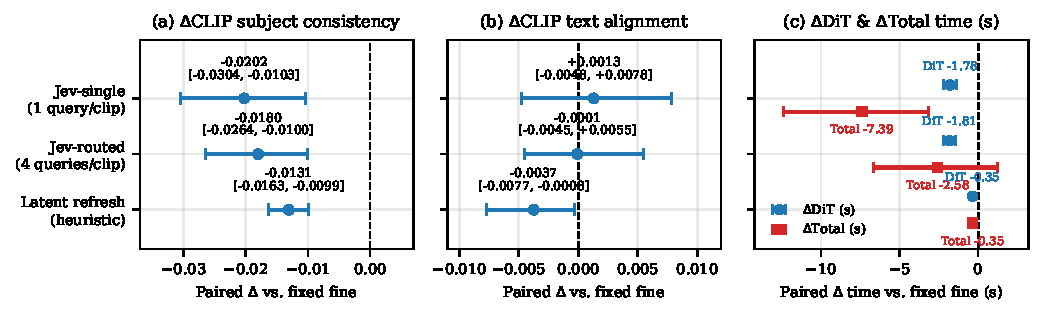
\includegraphics[width=0.90\textwidth]{fig_phase3_ci.pdf}
\caption{Confirmatory prompt-paired bootstrap differences against fixed fine (24 fresh A100 prompts, 10{,}000 resamples): (a) CLIP subject consistency, (b) CLIP text alignment, and (c) DiT and total latency. Both Jev policies pay a small, significant subject-consistency cost; text alignment is unchanged; the DiT and total-time savings are significant for the single-decision policy.}
\label{fig:phase3}
\end{figure*}

\subsection{A hold mode makes routing profitable on the T4}
\label{sec:hold}

Since the coarse mode is not cheaper on the T4, we add the genuinely cheap \emph{hold} mode and route with rule \eqref{eq:routing} (Table~\ref{tab:hold}, Fig.~\ref{fig:hold}). Two observations follow. First, routing ``moderate'' segments to coarse is counterproductive on this GPU---Jev-routed is worse than fixed fine on both axes, and its no-hold ablation is worse still---because coarse is slower \emph{and} less accurate there. Second, holding static segments is a better match than re-generating them: Jev-holdfine (static$\to$hold, else$\to$fine) beats fixed fine on both axes, with regret $-0.0010$, total time $-16.2$\,s ($-8.8\%$), and DiT time $-3.5$\,s ($-19\%$), at unchanged VAE cost. The margin is small and the sample is eight prompts, so we label this a weak positive; it matters because it isolates \emph{where} the saving comes from---a mode that is actually cheaper, not a signal trick.

\begin{figure*}[!t]
\centering
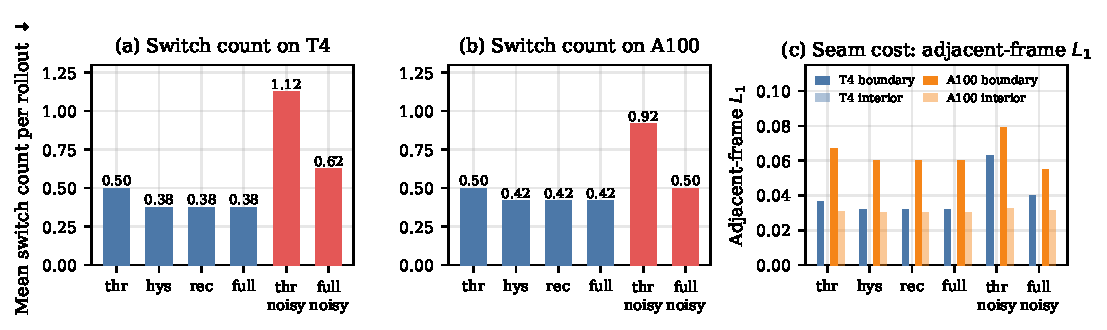
\includegraphics[width=0.90\textwidth]{fig_rq3.pdf}
\caption{Controller ablation (RQ3): mean switch count on (a) the T4 (8 prompts) and (b) the A100 (12 prompts), and (c) the seam cost---adjacent-frame $L_1$ at switch boundaries versus interior positions. Recovery plus hysteresis (\emph{full}) cuts switches on both GPUs, most clearly under injected $2\sigma_u$ signal noise, and reduces the noisy-arm seam cost.}
\label{fig:rq3}
\end{figure*}

\subsection{The A100 online arm: the endpoint rejects the hand-crafted policy}
\label{sec:a100online}

\begin{table*}[!t]
\centering
\caption{A100 online arms (57 frames, shared coarse prefix). Left: corrected policy set (12 prompts); the adaptive warp policy passes the internal gate but fails the independent endpoint and the total-time budget. Right: Jev policies with real in-loop oracle calls (12 prompts); Jev time is included in total time.}
\label{tab:a100online}
\renewcommand{\arraystretch}{1.12}
\begin{tabular}{@{}lrrrrr@{\hspace{2em}}lrrrr@{}}
\toprule
\multicolumn{6}{@{}l}{Policy set with hand-crafted signal} & \multicolumn{5}{l}{Jev policy set} \\
\cmidrule(r{2em}){1-6}\cmidrule{7-11}
Policy & refL1$\downarrow$ & DiT (s) & Total (s) & CLIP$\uparrow$ & warp$\downarrow$ & Policy & refL1$\downarrow$ & DiT (s) & Total (s) & CLIP$\uparrow$ \\
\midrule
fixed coarse  & 0.2728 & 2.55 & 45.5 & 0.9430 & 0.0435 & Jev-difficulty & 0.2678 & 3.19 & 47.7 & 0.9545 \\
fixed fine    & 0.2832 & 3.95 & 46.8 & \textbf{0.9836} & \textbf{0.0217} & Jev-routed     & 0.2715 & 2.04 & 33.7 & 0.9614 \\
fixed hold    & 0.2674 & \textbf{0.77} & \textbf{12.5} & 0.9926 & 0.0223 & Jev-holdfine   & 0.2739 & 2.59 & 34.9 & \textbf{0.9796} \\
random-50     & 0.2789 & 3.24 & 46.2 & 0.9588 & --- & fixed fine (ref) & 0.2832 & 4.01 & 41.8 & 0.9774 \\
adaptive warp & 0.2733 & 2.85 & 52.3 & 0.9492 & 0.0394 & fixed hold (ref) & 0.2674 & 0.76 & 11.5 & 0.9900 \\
\bottomrule
\end{tabular}
\end{table*}

On the A100 the cost gap is real, so the online test is informative (Table~\ref{tab:a100online}, Fig.~\ref{fig:a100online}). The adaptive warp policy passes the \emph{internal} gate ($+3.5\%$ refL1, $-27.9\%$ DiT, beating random same-budget), but the independent endpoint reverses the verdict: CLIP subject consistency $0.9492$ vs.\ $0.9836$ for fixed fine, and the signal's extra VAE decodes push total wall-clock above fixed fine ($52.3$ vs.\ $46.8$\,s). A second hazard appears here: on the A100 split the internal reference flatters the \emph{coarse} family (fixed coarse refL1 $0.2728$ $<$ fixed fine $0.2832$), the opposite direction from the T4---a diagnostic endpoint cannot be trusted in either direction, and precondition P3 binds on both GPUs.

The Jev policies, queried in-loop, behave differently. All Jev variants beat the random same-budget control; Jev-holdfine nearly matches fixed fine on the independent endpoint ($0.9796$ vs.\ $0.9774$) at $-35.5\%$ DiT and $-16.6\%$ total, and Jev-routed reaches $-49\%$ DiT at a larger quality cost. The oracle itself costs $\approx$1.0\,s per rollout including retries, with BLIP captioning at $0.18$--$0.70$\,s off the DiT path. A pilot then shows the \emph{single-decision} variant (one oracle query per prompt, reused across segments) cuts in-loop Jev time from $0.97$\,s to $0.24$\,s per rollout, while a free latent-space proxy signal is rejected (CLIP $0.9804$ vs.\ $0.9929$).

\begin{figure*}[!t]
\centering
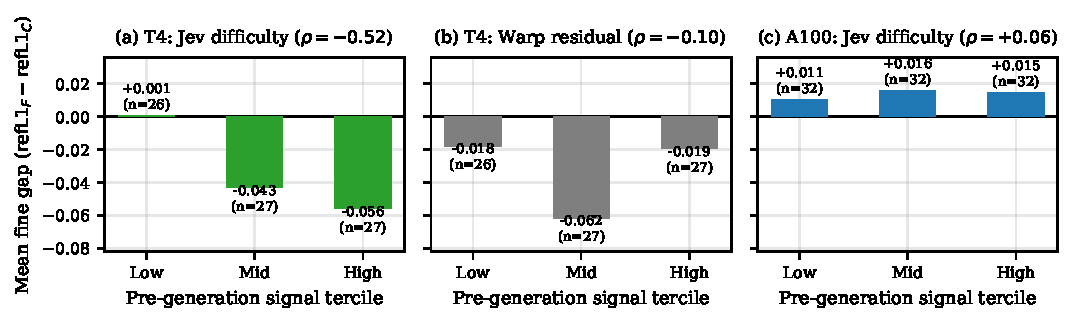
\includegraphics[width=0.88\textwidth]{fig_rq4.pdf}
\caption{Fine-versus-coarse gap across signal terciles. (a) On the T4 with the Jev difficulty signal the fine benefit grows monotonically with difficulty (Spearman $\rho = -0.517$ between difficulty and refL1$_F - $refL1$_C$; negative gap favors fine). (b) The hand-crafted warp signal shows no monotone relationship ($\rho = -0.099$; the mid tercile peaks). (c) On the A100 diagnostic split the same Jev signal is flat ($\rho = +0.059$), because the internal reference there favors the coarse family.}
\label{fig:rq4}
\end{figure*}

\subsection{Confirmatory study: a trade-off, not dominance}
\label{sec:phase3}

\begin{table*}[!t]
\centering
\caption{Confirmatory study: prompt-paired bootstrap differences against fixed fine (24 fresh A100 prompts, 10{,}000 resamples, 95\% CIs). Significant intervals are bold. The single-decision Jev policy is a genuine quality--cost trade-off; it is not dominant.}
\label{tab:phase3}
\renewcommand{\arraystretch}{1.12}
\begin{tabular}{@{}lcccc@{}}
\toprule
Policy & $\Delta$CLIP subj.\ cons. & $\Delta$CLIP text align. & $\Delta$DiT (s) & $\Delta$Total (s) \\
\midrule
Jev-single & $\mathbf{-0.0202}\ [-0.0304, -0.0103]$ & $+0.0013\ [-0.0048, +0.0078]$ & $\mathbf{-1.78}\ [-2.20, -1.37]$ & $\mathbf{-7.39}\ [-12.39, -3.16]$ \\
Jev-routed & $\mathbf{-0.0180}\ [-0.0264, -0.0100]$ & $-0.0001\ [-0.0045, +0.0055]$ & $\mathbf{-1.81}\ [-2.20, -1.41]$ & $-2.58\ [-6.62, +1.26]$ \\
latent refresh & $\mathbf{-0.0131}\ [-0.0163, -0.0099]$ & $-0.0037\ [-0.0077, -0.0003]$ & $-0.35\ [-0.36, -0.34]$ & $-0.35\ [-0.43, -0.26]$ \\
\bottomrule
\end{tabular}
\end{table*}

The confirmatory arm runs the single-decision Jev policy on 24 fresh prompts with prompt-paired bootstrap intervals (Table~\ref{tab:phase3}, Fig.~\ref{fig:phase3}). The honest reading is a trade-off: Jev-single saves $1.78$\,s of DiT time $[-2.20, -1.37]$ and $7.39$\,s of total time $[-12.39, -3.16]$---both significant---at a small significant loss of $-0.0202$ $[-0.0304, -0.0103]$ in CLIP subject consistency; text alignment is unchanged. Jev-routed saves the same DiT time without a significant total-time gain. Signal accuracy alone does not certify the system; the independent endpoint is what turns the saving into a measured price.

\begin{figure*}[!t]
\centering
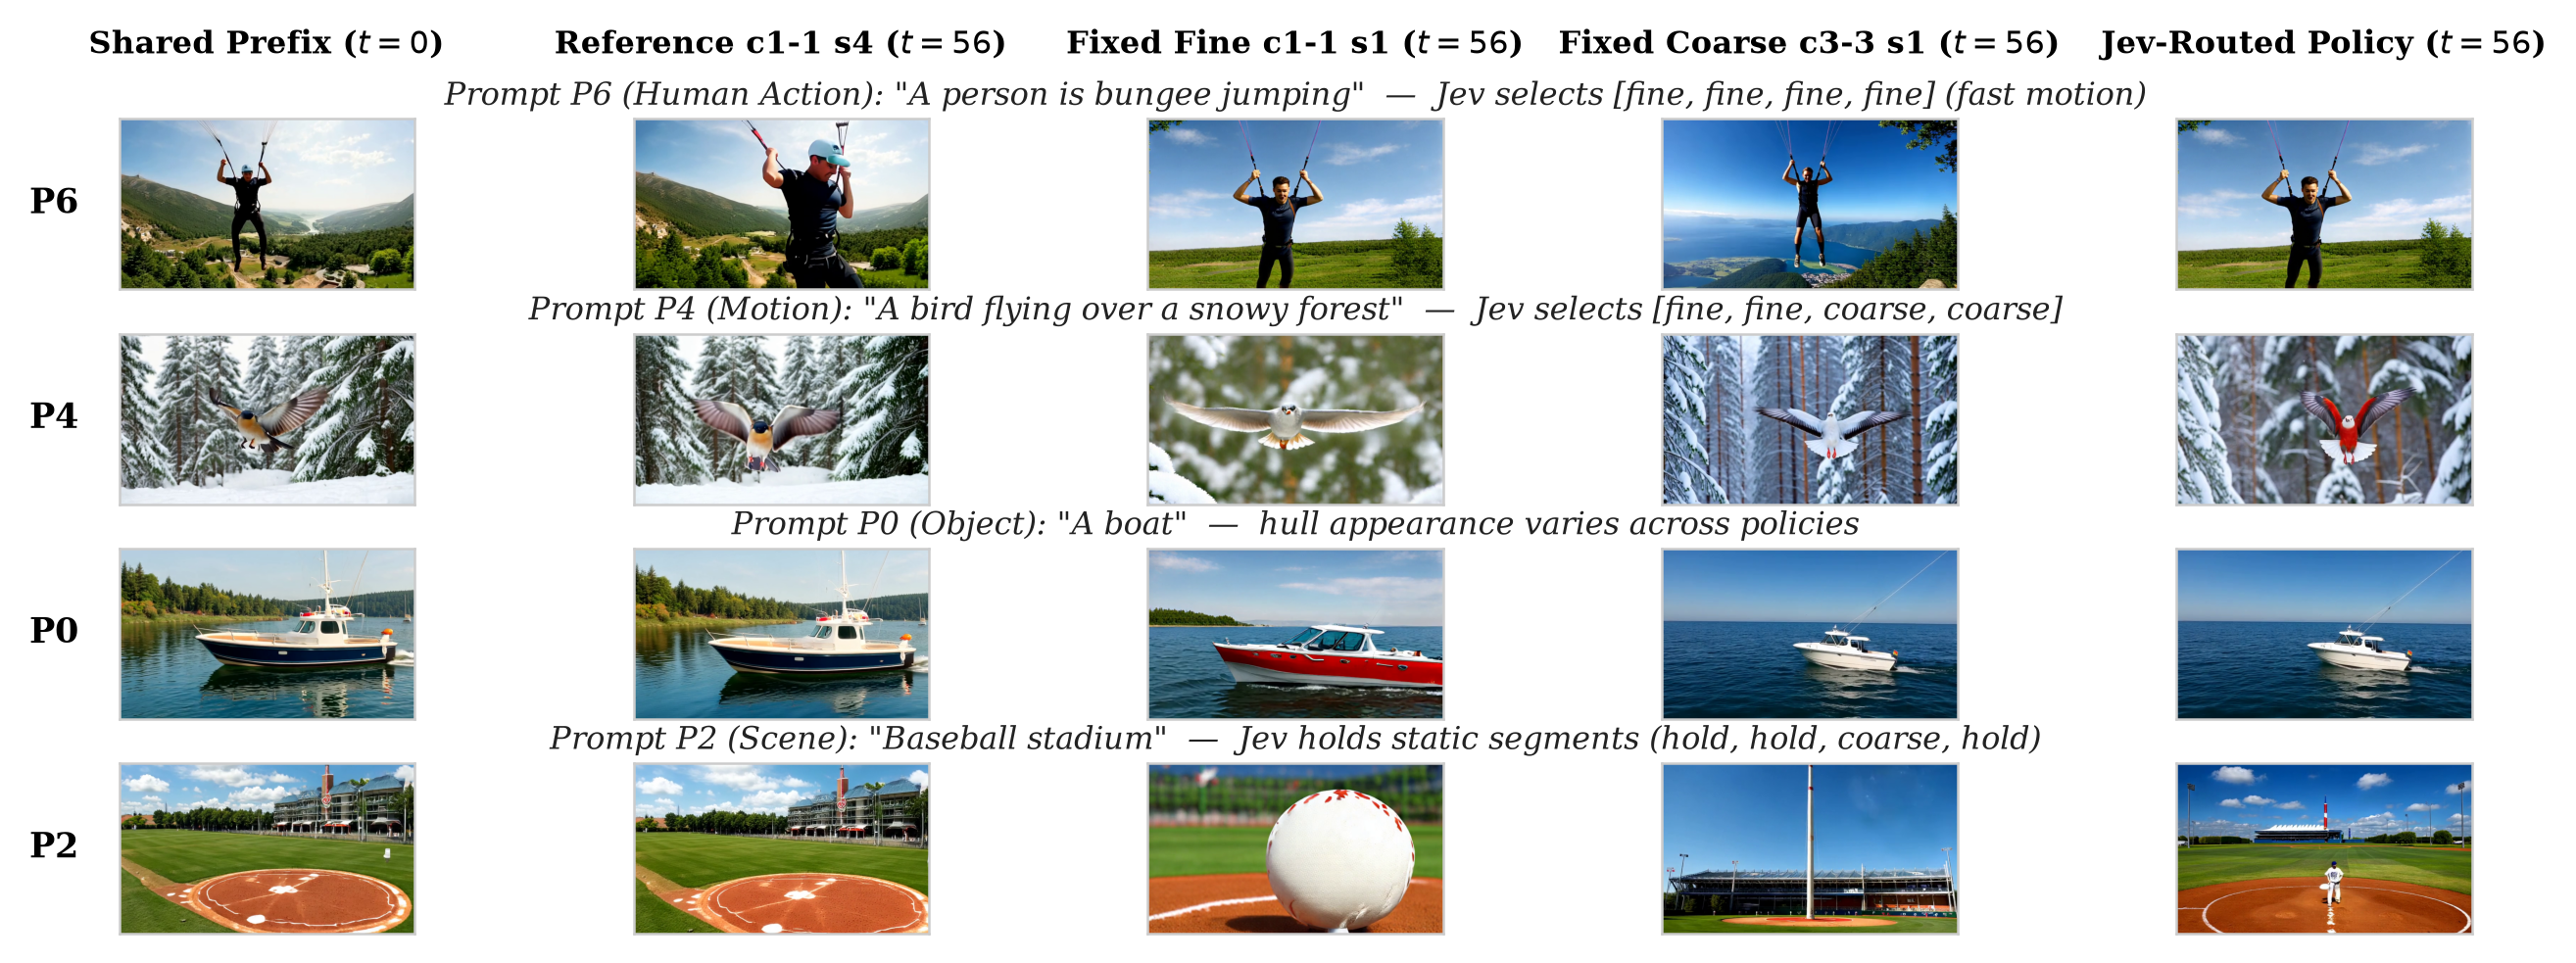
\includegraphics[width=0.90\textwidth]{qualitative_grid.png}
\caption{Representative decoded frames from matched 57-frame T4 rollouts for four prompts. Each column is the shared prefix frame ($t{=}0$), the \cfine{} four-step reference, fixed fine, fixed coarse, and the Jev-routed policy, all at $t{=}56$. Row P6 (a person bungee jumping) is routed to fine for all four segments and preserves the subject; row P4 (a bird over snow) mixes fine and coarse and shows coarse identity drift; row P0 (a boat) shows hull-appearance drift across policies; row P2 (a baseball stadium) is held on its static segments. These images are qualitative evidence only; every claim in the paper uses the numeric audits and the independent endpoints.}
\label{fig:qual}
\end{figure*}

\subsection{Recovery and hysteresis stabilize switching on both GPUs (RQ3)}
\label{sec:rq3}

\begin{table}[!t]
\centering
\caption{Controller ablation (RQ3). Switches are per rollout (four decisions, T4 / A100). AUH is area-under-horizon refL1 regret; seam/interior are adjacent-frame $L_1$ at switch boundaries and interior positions. Paired differences are full minus threshold-only.}
\label{tab:rq3}
\renewcommand{\arraystretch}{1.12}
\footnotesize
\setlength{\tabcolsep}{3.5pt}
\begin{tabular}{@{}llcccc@{}}
\toprule
GPU & Controller & switches$\downarrow$ & AUH$\downarrow$ & terminal$\downarrow$ & seam\,/\,interior \\
\midrule
\multirow{4}{*}{T4}
 & threshold-only      & 0.50 & 0.3133 & 0.3171 & 0.0364\,/\,0.0280 \\
 & \textbf{full}       & \textbf{0.38} & \textbf{0.3116} & \textbf{0.3104} & 0.0321\,/\,0.0273 \\
 & threshold (noisy)   & 1.12 & 0.3159 & 0.3172 & 0.0630\,/\,0.0290 \\
 & \textbf{full (noisy)} & \textbf{0.62} & \textbf{0.3150} & \textbf{0.3139} & 0.0399\,/\,0.0260 \\
\midrule
\multirow{4}{*}{A100}
 & threshold-only      & 0.50 & 0.2767 & 0.2955 & 0.0672\,/\,0.0305 \\
 & \textbf{full}       & \textbf{0.42} & 0.2772 & 0.2977 & 0.0601\,/\,0.0303 \\
 & threshold (noisy)   & 0.92 & 0.2741 & 0.2997 & 0.0793\,/\,0.0326 \\
 & \textbf{full (noisy)} & \textbf{0.50} & \textbf{0.2718} & \textbf{0.2921} & 0.0551\,/\,0.0315 \\
\bottomrule
\end{tabular}
\end{table}

Table~\ref{tab:rq3} and Fig.~\ref{fig:rq3} ablate the controller on both GPUs with a switch-producing calibration ($\tau$ at the pooled development median, $\Lambda = 2\sigma_u$, $R{=}2$). Recovery plus hysteresis reduces switching without worsening regret: on the T4, $0.50 \rightarrow 0.38$ switches with area-under-horizon (AUH) regret $-0.0017$ and terminal regret $-0.0067$; under injected $2\sigma_u$ noise, $1.12 \rightarrow 0.62$ ($-45\%$). On the A100, $0.50 \rightarrow 0.42$ on the real signal and $0.92 \rightarrow 0.50$ ($-45\%$) under noise, with AUH regret essentially unchanged ($+0.0005$). The mechanism's premise---that switching has a cost---is directly measured: adjacent-frame $L_1$ at switch boundaries exceeds interior positions ($0.0364$ vs.\ $0.0280$ on the T4; $0.0672$ vs.\ $0.0305$ on the A100, $0.0793$ under noise), and the full controller reduces the noisy boundary cost ($0.0630 \rightarrow 0.0399$ T4; $0.0793 \rightarrow 0.0551$ A100). On the near-monotone real traces the $\Lambda \in \{0.5,1,2,4\}\sigma_u$ and $R \in \{1,2,3\}$ sweeps are flat, so the benefit is observable mainly under signal noise; we report it as such. RQ3 is supported on both GPUs, consistent with the oscillation bound.

\subsection{Monotonicity is signal- and endpoint-dependent (RQ4)}
\label{sec:rq4}

The exploratory RQ4 asks whether the fine-versus-coarse benefit is monotone in the pre-generation signal. On 80 paired T4 segments, the warp signal gives $\rho = -0.099$ with non-monotone terciles ($-0.0225, -0.0571, -0.0195$); the Jev difficulty signal on the same segments flips the result to monotone ($\rho = -0.517$; terciles $+0.0006, -0.0430, -0.0558$; Fig.~\ref{fig:rq4}), and the relation holds within both horizons (57 frames: $\rho=-0.458$; 81 frames: $\rho=-0.581$). The earlier non-monotonicity was therefore a \emph{signal-quality artifact}, not a property of the modes. On the A100 confirmatory split, however, the same Jev signal gives $\rho = +0.059$ (AUROC $0.451$): no relationship. This is confounded rather than a clean disconfirmation---on that split the internal reference favors coarse (mean fine gap $+0.0137$; only $38.5\%$ of segments favor fine), so the label carries no stable fine benefit to track. RQ4's verdict is thus \emph{signal- and endpoint-dependent}: monotone with a good oracle against a fine-leaning reference, flat against a coarse-leaning one---the sharpest illustration of why P2 and P3 must be audited together.

\subsection{Qualitative evidence}
\label{sec:qual}

Figure~\ref{fig:qual} shows matched frames across policies: for a fast-motion human-action prompt the fixed coarse rollout drifts to a different person over a different background while fixed fine and the Jev-routed rollout preserve the subject, and for a bird-over-forest prompt the coarse rollout loses subject identity. We treat these as visual context for the metrics, not as evidence.

\section{Discussion}
\label{sec:discussion}

The audit separates three claims that are easy to merge. \emph{Cost} is a hardware question: the \ccoarse{} family amortizes a longer temporal stride over fewer, heavier forwards, and whether that trade pays is decided by the per-forward ratio against the schedule's break-even point \eqref{eq:breakeven}---$3.01$ versus $1.60$ here. NFE is not GPU time, and any adaptive-granularity proposal should verify the wall-clock gap at matched quality on the target GPU before building a controller on top of it. \emph{Signal} is a content question: four hand-crafted statistics of the pre-decision context all fail a locked held-out test, while a text-only System One model that reads a caption and motion summary succeeds---and does so before generation, off the GPU, at sub-second latency. The bottleneck was signal content, not threshold tuning. \emph{Endpoint} is a measurement question: the internal reference reversed its fine/coarse preference between the T4 and A100 splits, and the A100 online arm shows a policy that ``passes'' internally while losing subject consistency and total time. Independent endpoints are not optional in this setting.

For practitioners, the procedure is simple: measure the per-forward ratio against the schedule break-even on the deployment GPU; if no gap exists, route between fine and a genuinely cheap hold mode rather than a heavier coarse chunk; drive the router with an off-GPU oracle rather than a lagged decoded probe; and wrap the switch in hysteresis and recovery, because the seam cost is real and noise-driven flips are suppressible by the band. The Jev-holdfine policy is the deployed form on the T4, and the single-decision Jev policy on the A100, where coarse re-enters the action set because the cost gap exists there.

\section{Reproducibility}
\label{sec:repro}

Every quantitative claim resolves to a per-run audit record produced by a named script, and the raw rows, generated videos, locked manifests, and calibration freezes are retained with the run inventory. The two GPUs, checkpoint names, frozen splits, calibration constants, and statistics are stated in Section~\ref{sec:setup}; negative results are preserved rather than edited out. The complete source tree, figure-generation scripts, and run metadata are released in the public repository \url{https://github.com/j1s4nn/jev-adaptive-granularity-WM}, so that the cost, signal, and endpoint audits can be repeated and independently verified on new hardware, which is the study's central recommendation.

\section{Limitations}
\label{sec:limitations}

Several limitations bound the claims. (i) Samples are small and single-seeded: three development prompts for the sweeps, eight fresh prompts for the T4 online, controller, and Jev studies, and twelve and twenty-four fresh prompts for the A100 arms; the results have no confirmatory power for a universal claim, and the confirmatory intervals are prompt-paired over $n{=}24$. (ii) The Jev oracle is external, proprietary, and versioned (\texttt{jev-latest}); results depend on its continued behavior, its input is a BLIP caption plus motion statistics of the pre-decision frame (caption noise propagates to the signal), and its AUROC rests on 80 segments from eight prompts with wide intervals. (iii) RQ2 is a trade-off, not dominance: the confirmatory savings and the $-0.020$ subject-consistency loss are both significant. (iv) The internal refL1 reference is a fine-family diagnostic whose direction flips between datasets; the independent CLIP and classical endpoints are the safeguard, but CLIP text alignment on short prompts is noisy, and we report no FVD, PSNR, LPIPS, or full VBench suite because no ground-truth video exists for these rollouts. (v) The study is text-to-video only---no action-conditioned checkpoint was available, the action-potential weight $\lambda$ is zero throughout, and the EMA uncertainty signal planned in the proposal was unavailable in the verified checkpoints. (vi) Total wall-clock on the T4 is dominated by mode-independent VAE decode; the mode-dependent cost is DiT time, and other backbones or more throughput-bound hardware could shift the ratio. (vii) The fixed-mode-suboptimality proposition's parameter regime was never reachable in deployment; the propositions are retained as motivation.

\section{Conclusion}
\label{sec:conclusion}

Adaptive temporal granularity in a causal video world model is neither a free win nor a fiction---it is a conditional trade-off whose conditions this paper makes explicit. The cost precondition is a property of the GPU: the chunk-3 coarse mode of Causal-rCM is slower than frame-wise fine generation on a T4 yet $1.46\times$ faster in DiT time on an A100. The signal precondition is a property of the signal content: a preregistered hand-crafted suite fails on locked data (AUROC $0.491$), while the Jev System One oracle predicts coarse-unsafe segments at AUROC $0.788$ in $0.67$\,s off the generation path. The endpoint precondition is a property of the evaluation: the internal reference flatters different families on different splits, and only the independent endpoints turn the A100 savings into a measured, significant price. Within those conditions, the mechanism of the title works: Jev-routed granularity with a hysteresis band and a recovery window cuts switches by up to $45\%$ without worsening regret on both GPUs, routes static segments to a hold mode that beats fixed fine on both quality and cost on the T4, and delivers a significant DiT and total-time saving at a small significant subject-consistency cost on the A100. Future work should verify cost gaps at matched quality before building controllers, prefer genuinely cheap modes over heavier coarse chunks, move uncertainty estimation off the GPU, and extend the audit to action-conditioned rollouts, larger held-out studies, blinded human evaluation, and FlashAttention-class hardware.

\bibliographystyle{IEEEtran}
\bibliography{references_ieee}

\end{document}
